%% LyX 2.2.4 created this file.  For more info, see http://www.lyx.org/.
%% Do not edit unless you really know what you are doing.
\documentclass[english]{article}
\usepackage{lmodern}
\usepackage[T1]{fontenc}
\usepackage[latin9]{inputenc}
\usepackage{geometry}
\geometry{verbose,tmargin=3cm,bmargin=3cm,lmargin=2.5cm,rmargin=2.5cm}
\usepackage{textcomp}
\usepackage{graphicx}
%\usepackage{mcode}

\renewcommand\thesection{\alph{section}}

\makeatletter

%%%%%%%%%%%%%%%%%%%%%%%%%%%%%% LyX specific LaTeX commands.
%% Because html converters don't know tabularnewline
\providecommand{\tabularnewline}{\\}

\makeatother

\usepackage{babel}

\usepackage{pdfpages}
\usepackage{amsmath}


\begin{document}

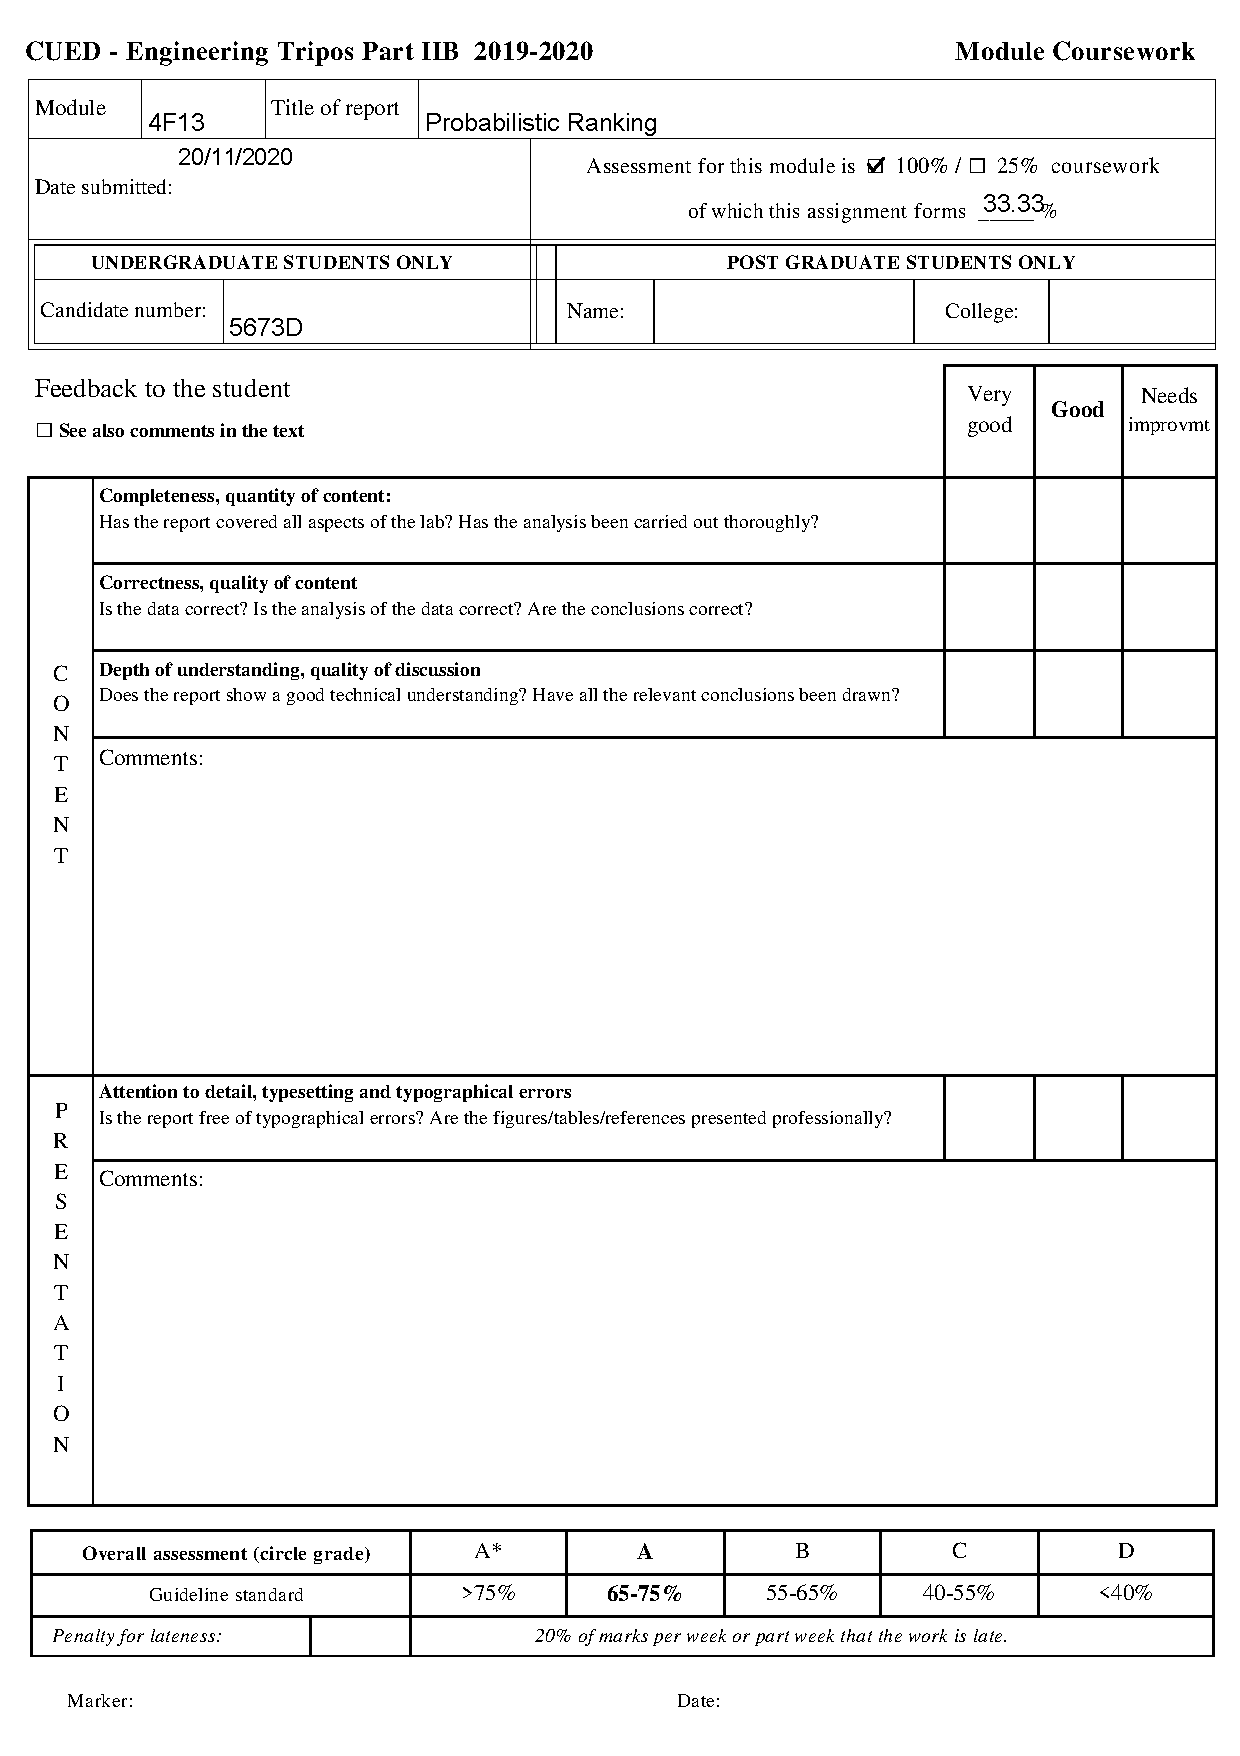
\includepdf{cover.pdf}
\title{4F13: Probabilistic Machine Learning\\
Probabilistic Ranking}

\author{Candidate number: 5673D \\
		Words count: approximetly 990
	}

\maketitle

\section{Gibbs sampling for the TrueSkill model \label{a}}
	
	
     We want to compute probabilistic rankings of the skill of 2011 ATP players. To do this, we will make use of the data form \texttt{tennis\_data.mat}, which consists of an array $\mathbf{W}$ of $ 107 $ players and a matrix $\mathbf{G}$ of $ 1801 $ games and their outcomes. First, we will have a look at the first algorithm presented in lectures, Gibbs sampling in TrueSkill. And we start by feeling the missing code with the following computation of the mean of the conditional skill distribution and the precision matrix.
	
	In the lectures, the following formulas were presented:
	
	\begin{equation}
		[\Sigma^{-1}]_{ii} = \sum_{g=1}^{G} \delta(i-I_g) +\delta(i-J_g)
	\end{equation}
\begin{equation}
	[\Sigma^{-1}]_{i\neq j} = -\sum_{g=1}^{G} \delta(i-I_g)\delta(j - J_g)+\delta(j-I_g)\delta(i-J_g)
\end{equation}
\begin{equation}
	\mu_i = \sum_{g=1}^{G} \delta(i-I_g) - \delta(i-J_g)
\end{equation}

Note that we used the same implantation and iterate over players and then after games to compute the mean. But this can be done in a similar easier fashion as we implemented the precision matrix. We can iterate over the games and update the matrix's indices.

\begin{verbatim}
%Compute mean of the conditional skill distribution	

for p = 1:M
    m(p) = 0;
    for g = 1:N
        if( p == G(g,1))
            m(p) = m(p) + t(g);
        elseif (p == G(g,2))
            m(p) = m(p) - t(g);
        else
            continue
        end
    end
end

%Compute iS matrix
for g = 1:N
    I = G(g,1);
    J = G(g,2);
    iS(I,I) = iS(I,I) + 1;
    iS(J,J) = iS(J,J) + 1;
    iS(I,J) = iS(I,J) - 1;
    iS(J,I) = iS(J,I) - 1;
end
\end{verbatim}

Now, we are finally able to draw samples from the conditional skill distribution. Although, we can draw samples from the distribution we still do not have the skill of each player. To find the skill we will compute the mean of th samples up to the current iteration:

\begin{equation}
	\mu(n) = \frac{1}{n}\sum_{i=1}^{n} sample_i
\end{equation}

We now that this Monte Carlo estimator of the mean tends to the true mean as n tends to infinity. Therefore, in Figure \ref{fig:predictive_distributions} on the left we plot the values of the mean as function of the number of iterations for 4 different players. This figure shows an increase behaviour for the mean for the first $ 100 $ iteration, after which it is reaching a plateau. We call these first $ 100 $ iterations the burn-in time of the Gibbs sampling, the time it takes for the sampled chained to converge to the desired distribution, In practice, we when calculating the mean, we will take into consideration only the samples from the 100th iteration onward.

	\begin{figure}[h]
		\begin{centering}
			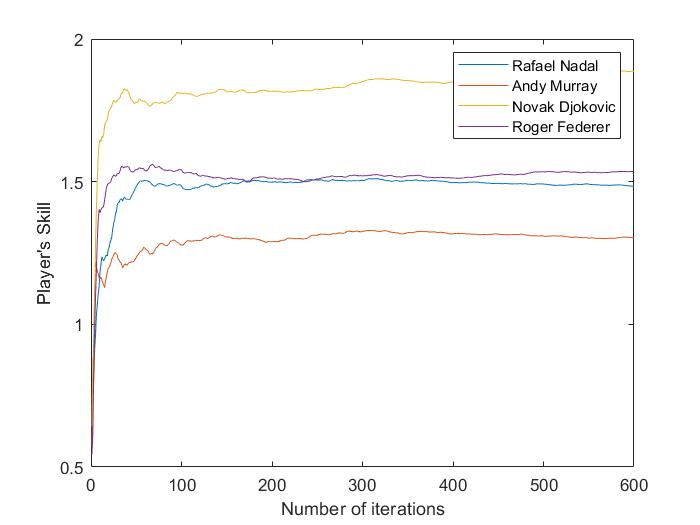
\includegraphics[width=0.3\paperwidth]{2a.jpg}\hspace{1cm}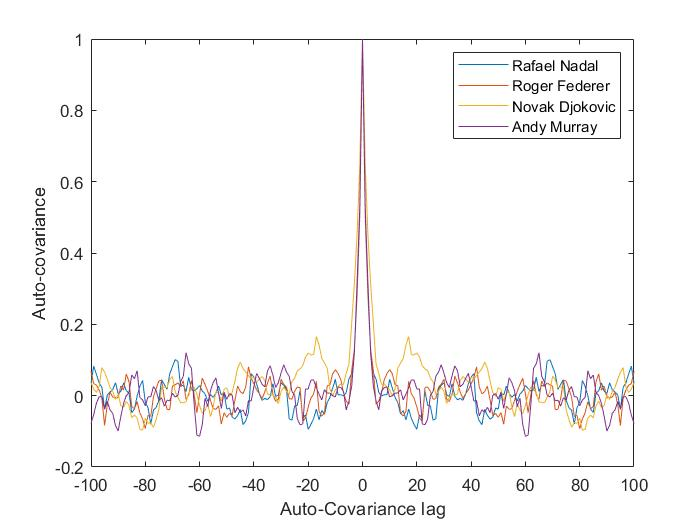
\includegraphics[width=0.3\paperwidth]{2ab.jpg}
			\par\end{centering}
		\caption{ On the left: The average skill of the top 4 players after each iterations. On the right: the covariance between skill distribution samples.   
		 \label{fig:predictive_distributions} }
	\end{figure}

Taking our investigation one step further, we can now look at the auto-covariance function of the samples drawn, Figure \ref{fig:predictive_distributions} on the right. This Figure shows a strong correlation between around $ 10 $ consecutive samples and this will slow down our process of inferring the true mean. As a solution, we can take into consideration every 10th sample.
  

\section{Inference of the skill using message passing and EP }

In this section, we will infer our skill by using message passing and EP. This is based on the sum-product rule an it uses tress consisting of values and factor to approximate the marginal distribution of the skill. In this algorithm the messages are updated iteratively from the neighbour values, making the computations localized. 


In Figure \ref{fig:ep}, we can see the it archives converges of the marginal distribution of the skills in relatively few iteration.  

\newpage

\begin{figure}
	\begin{centering}
		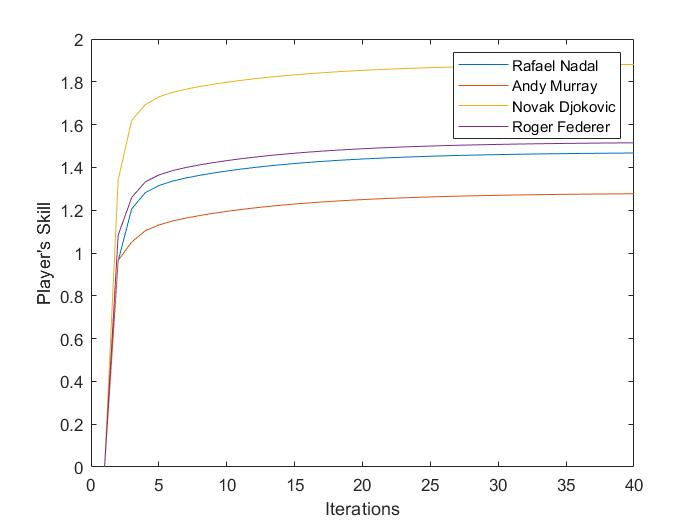
\includegraphics[width=0.5\paperwidth]{2b.jpg}
		\par\end{centering}
	\caption{Player skill vs number of iterations.\label{fig:ep} }
\end{figure}


\section{Probabilities of higher skill and game outcome}

In this section, we will use the marginal distribution of the skill from our message passing algorithm to calculate the probability of one player's skill being higher than the other and the probability of the outcome of the game. In particular we will have a look at the top 4 players (Novak Djokovic, Roger Federer, Rafael Nadal and Andy Murray). 

Let us have a look on how to calculate the probability of Player 1 having a higher skill than Player 2, given the mean and variances of both players skills $ (\mu_i, \sigma^2_i) $, $ i={1,2} $.

\begin{equation}
	p(w_1 > w_2) = \mathcal{Q} \left( \frac{\mu_2 - \mu_1}{\sqrt{\sigma_1^2 + \sigma^2_2}} \right)
\end{equation}

As for probability of Player 1 winning against Player 2, we have to account for performance inconsistency and we need to add noise to our skill difference. This will result to the following:

\begin{equation}
	p(\text{Player 2 wins}) = \mathcal{Q} \left( \frac{\mu_2 - \mu_1}{\sqrt{1+\sigma_1^2 + \sigma^2_2}} \right)
\end{equation} 


  
\begin{table}[h]
	\centering{}%
	\begin{minipage}[t]{0.5\textwidth}%
		\begin{center}
			\begin{tabular}{cc |c|c|c|}
				& Djo & Nad & Fed & Mur\tabularnewline
				\cline{2-5} 
				Djo & - & 0.94 & 0.91  & 0.98\tabularnewline
				\cline{2-5} 
				Nad & 0.06 & - & 0.43  & 0.77\tabularnewline
				\cline{2-5} 
				Fed & 0.09 & 0.57 & -  & 0.91\tabularnewline
				\cline{2-5} 
				Mur & 0.02 & 0.23 & 0.19  & -\tabularnewline
				\cline{2-5} 
				
			\end{tabular} 
			\par\end{center}
		\caption{Probabilities of one player skill being higher than the other \label{tab:skill}}
		%
	\end{minipage}%
	\begin{minipage}[t]{0.5\textwidth}%
		\begin{center}
			\begin{tabular}{cc |c|c|c|}
				& Djo & Nad & Fed & Mur\tabularnewline
				\cline{2-5} 
				Djo & - & 0.66 & 0.64  & 0.72\tabularnewline
				\cline{2-5} 
				Nad & 0.34 & - & 0.48  & 0.57\tabularnewline
				\cline{2-5} 
				Fed & 0.36 & 0.51 & -  & 0.59\tabularnewline
				\cline{2-5} 
				Mur & 0.28 & 0.43 & 0.41  & -\tabularnewline
				\cline{2-5} 
				
			\end{tabular}
			\par\end{center}
		\caption{Probabilities of a player winning a game\label{tab:wins}}
		%
	\end{minipage}
\end{table} 
 
 The resulting probabilities tables are shown above. As we expected from Figures \ref{fig:ep} There is a large skill gap between Djokovic and Federer and it is very improbable for Federer the have a better skill than Djokovic. Although, because of performance inconsistency Federer has a chance of $ 36\% $ to win the match. Same happens between Andy Murray and Rafael Nadal. The difference is between Federer and Nadal where the skill level is close and Federer has $ 60\% $ chance of having a better skill but the outcome of the game is $ 50\% $ with a slightly edge to Federer.
    
\section{Nadal vs Djokovic}

In this section, we will use again Gibbs sampling, but this time we only sample after 100th iteration and once every 10 iterations. This will give us good unbiased estimators for the mean and variance of the skill. We present the first two methods if Figure \ref{fig:nad} and the last one is looking at the last value of our mean estimator. We can easily exclude the last method as being the best as it is already embedded in the univariate Gaussians. And we propose the first comparison to be the best as we can see on the graph if the 2 Gaussians overlap(In this case they are not). Therefore, the chance for Nadal to have a better skill than Djokovic is very improbable.

\begin{figure}[h]
	\begin{centering}
		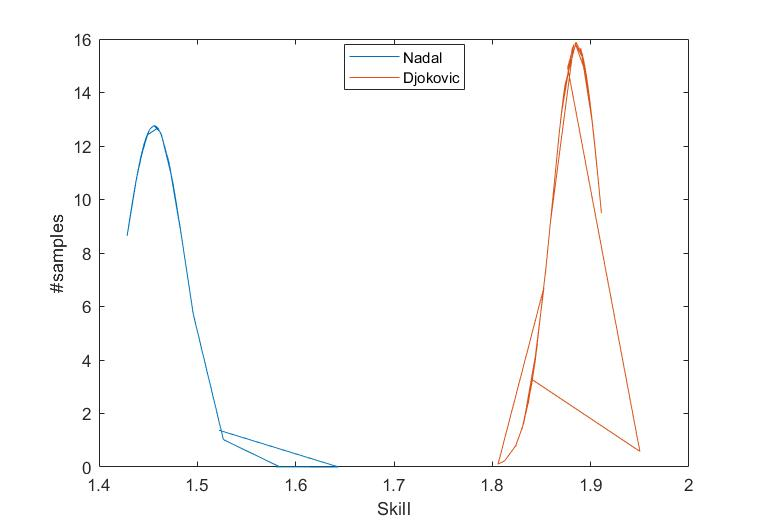
\includegraphics[width=0.3\paperwidth]{2d1.jpg}\hspace{1cm}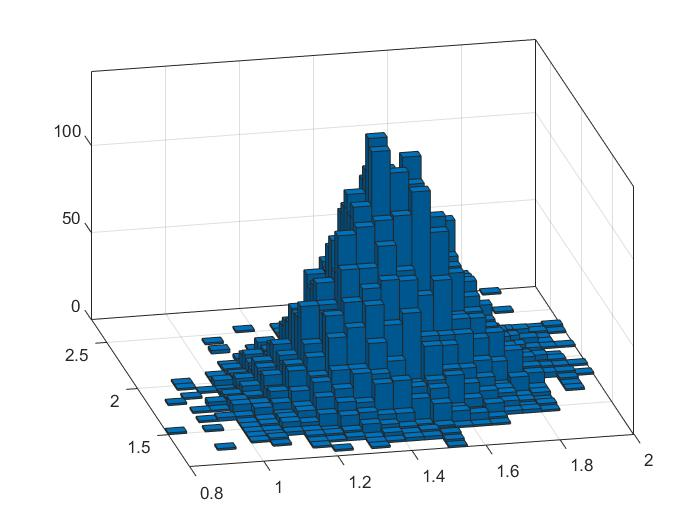
\includegraphics[width=0.3\paperwidth]{2d2.jpg}
		\par\end{centering}
	\caption{ Univariate Gaussians and Bivariate Gaussian for Nadal and Djokovic skills  
		\label{fig:nad} }
\end{figure}

We compute again the table of probabilities of one's player skill to be higher than another. There a high level of similarity between this one and the one previously seen using message passing. Djokovic still has the highest probability of being higher, but now there is a better difference between Federer and Nadal, and there is not a big difference between Federer and Murray any more.
\begin{table}[h]
			\begin{center}
		\begin{tabular}{cc |c|c|c|}
			& Djo & Nad & Fed & Mur\tabularnewline
			\cline{2-5} 
			Djo & - & 0.96 & 0.91  & 0.97\tabularnewline
			\cline{2-5} 
			Nad & 0.04 & - & 0.38  & 0.70\tabularnewline
			\cline{2-5} 
			Fed & 0.09 & 0.62 & -  & 0.77\tabularnewline
			\cline{2-5} 
			Mur & 0.03 & 0.30 & 0.23  & -\tabularnewline
			\cline{2-5} 
			
		\end{tabular}
		\par\end{center}
	\caption{Probabilities of a player skill being higher(Gibbs)\label{tab:wins}}
\end{table}

\newpage
\section{Players Ranking}

We know want to compare the ranking of the players using predicting outcomes for 3 different methods: Gibbs Sampling Figure \ref{fig:ov}, on the left, Message Passing, same Figure, on the right and Win Ratio, \ref{fig:ww}. The empirical win ratio makes it hard to determine which player has a better skill. The win ratio value is close, but each player's opponents are held out. In this scenario, Andy Murray appears to have performed better than Nadal. The other two models appear to be consisted, making the same ranking order. 

\begin{figure}[h]
	\begin{centering}
		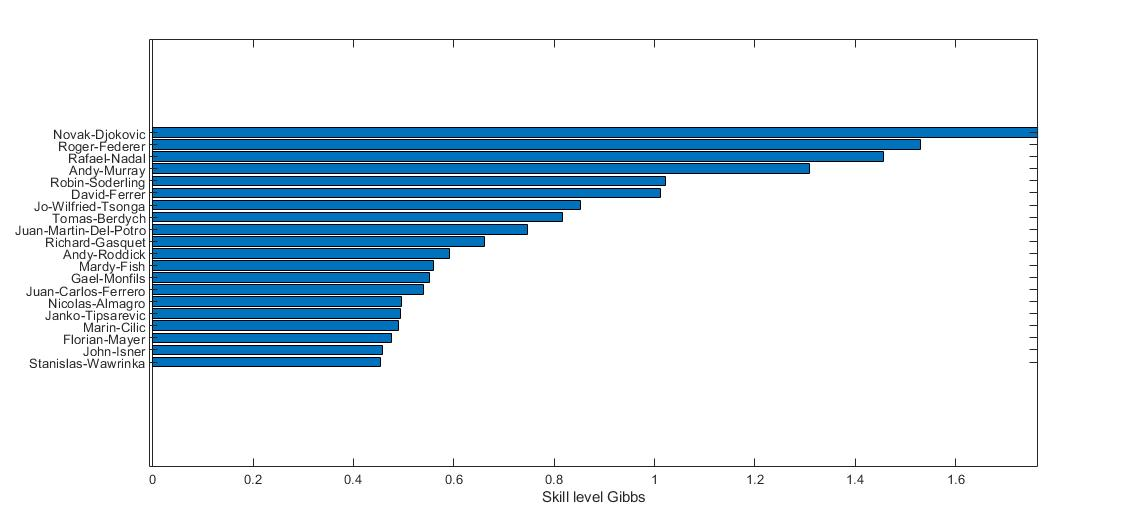
\includegraphics[width=0.3\paperwidth]{2em.jpg}\hspace{1cm}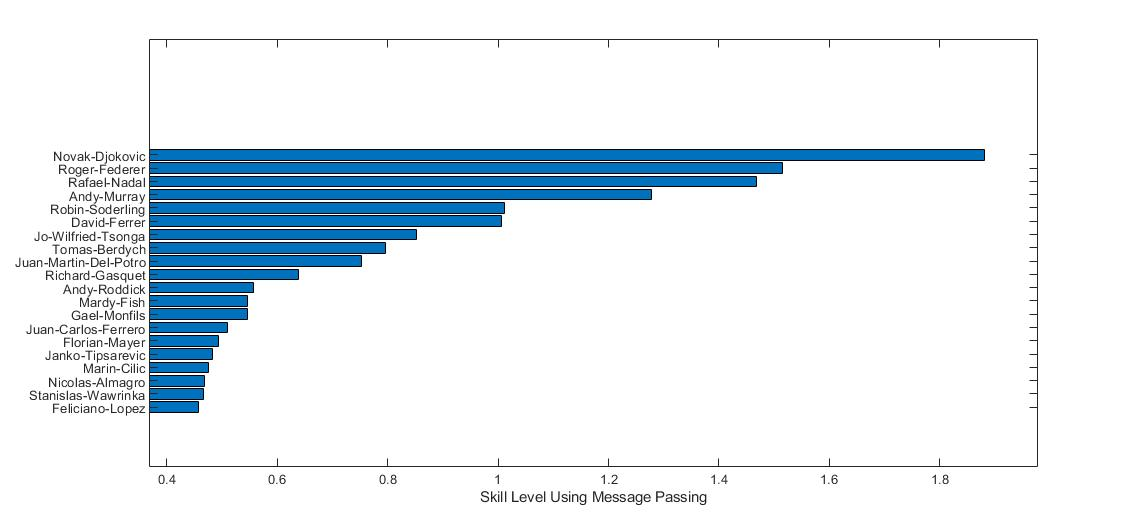
\includegraphics[width=0.3\paperwidth]{2eg.jpg}
		\par\end{centering}
	\caption{ Skill Levels
		\label{fig:ov} }
\end{figure}

\begin{figure}[h]
	\begin{centering}
		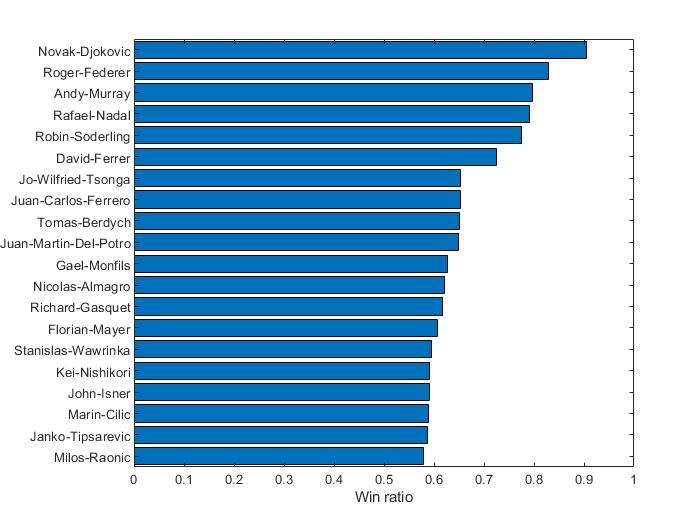
\includegraphics[width=0.3\paperwidth]{win.jpg}
		\par\end{centering}
	\caption{Win ratio.\label{fig:ww} }
\end{figure}

\end{document}
